\section{Turingmaschinen}\datenote{09.01.2019}
\newcommand{\M}{\mathcal{M}}
\newcommand{\godel}[1]{\ulcorner #1 \urcorner}
\newcommand{\D}{\mathcal{D}}
\newcommand{\mblank}{\text{\blank}}

\hide{
%\section{\acf{TM}}
1930er Jahre\\
Suche nach formalem Modell für maschinelle Berechenbarkeit
\begin{description}
	\item[Alan Turing:] (1912-1954) Turingmaschine 1936
	\item[Alonzo Church:] Lambdakalkül 1936
        \item[Emil Post:]  Postband 1936
	\item[Kleene, Sturgis:] partiell rekursive Funktionen
	\item[Chomsky:] Typ-0-Grammatiken 1956
\end{description}
\emph{Alan Turing:}\begin{minipage}[t]{.8\textwidth}
\begin{itemize}[parsep=0pt]
	\item Informatik, Logik
	\item Kryptographie (Enigma Entschlüsselung, Sprachverschlüsselung)
	\item KI (Turing-Test)
\end{itemize}\end{minipage}

außerdem: Turing-Award
}

Wir werden in diese Kapitel ein weiteres Maschinenmodell, das der \emph{Turingmaschine}~\footnote{Alan Mathison Turing *1912 †1954}, kennenlernen.
Im Gegensatz zu endlichen Automaten und Kellerautomaten
sind Turingmaschinen so ``mächtig''
dass die Arbeitsweise jeder Rechenmaschine durch eine Turingmaschine modelliert werden kann.

Diese ``Mächtigkeit'' stellt uns vor neue Herausforderungen:
Eine Turingmaschine kann nicht-triviale Endlosschleifen erlauben und wir werden im Allgemeinen 
nicht entscheiden können ob eine Berechnung überhaupt terminiert oder statt dessen unendlich lange läuft.

Die Turingmaschine basiert auf der Idee, dass man die Arbeitsweise eines rechnenden Menschen abstrakt und idealisiert wie folgt beschreiben könnte:
Wir bewegen uns mit einem Bleistift und einem Radiergummi auf einem Karopapier, das in alle Richtungen unbeschränkt ist 
(weil wir immer zusätzliches Papier anlegen könnten wenn der Seitenrand erreicht ist).
In jedem Rechenschritt lesen wir zunächst das Zeichen das in dem Kästchen unter der Bleistiftspitze steht.
Anschließend radieren wir das Zeichen aus, beschriften das Kästchen neu und Bewegen die Bleistiftspitze zu einem benachbarten Kästchen oder 
lassen die Position unverändert. 
Unser Gehirn hat nur endlich viele verschiedene Zustände und steuert welches Zeichen wir schreiben und wohin die Bleistiftspitze bewegt wird.
Der Zustand unseres Gehirns kann sich in jedem Rechenschritt ändern und wird auch durch das gelesene Zeichen beeinflusst.

Im Gegensatz zu diesem Modell eines rechnenden Menschen hat die Turingmaschine ein in beide Richtungen unbeschränktes Band statt eines Karopapieres und einen Schreib- Lesekopf statt Bleistift und Radiergummi.


\subsection{Turingmaschine \normalfont(informell)}

Die \acf{TM} ist eine Erweiterung des endlichen Automaten mit den folgenden Zusätzen.
\begin{itemize}
	\item Die Eingabe steht auf einem Band, das rechts und links der Eingabe unendlich viele Zellen hat.
	
	\begin{figure}[H]\centering
		\begin{tikzpicture}[every node/.style={block}]
			\node (1) {\blank};
			\node (2) [right=of 1] {b};
			\node (3) [right=of 2] {a};
			\node (4) [right=of 3] {n};
			\node (5) [right=of 4] {a};
			\node (6) [right=of 5] {n};
			\node (7) [right=of 6] {e};
			\node (8) [right=of 7] {\blank};
			\node (9) [right=of 8] {\blank};
			\node (10) [right=of 9] {\blank};
			\node (11) [right=of 10] {\blank};
			\node (last) [right=of 11] {\blank};
			
			\node (Kopf) [below=1.5em of 2, draw=none, text height=.5em] {Kopf}
			edge [->, shorten >=.5ex, semithick] (2);
			
			\node (TB) [below=.5em of 9, draw=none, text height=.5em,  anchor=north west] {Turingband};
			
			\draw (8.south) -- ($(8.south)-(0,1em)$) -- ($(TB.north west)-(0,.5em)$);
			
			% Open begin and end.
			\draw (1.north west) -- ++(-1cm,0) (1.south west)
			-- ++ (-1cm,0) (last.north east)
			-- ++ ( 1cm,0) (last.south east)
			-- ++ ( 1cm,0);
		\end{tikzpicture}
		\vspace{-1em}
		\caption{Turingband}
		% 	\framebox{q} = Zustand
	\end{figure}
	
	\item Der Kopf der \ac{TM} kann nicht nur Zeichen lesen, sondern auch Zeichen schreiben.
	Der Kopf steht wie bei endlichen Automaten immer auf genau einer Zelle und liest in jedem Rechenschritt das Zeichen, welches auf dieser Zelle geschrieben steht.
	Im Gegensatz zu endlichen Automaten kann der Kopf aber auch Zeichen schreiben; er tut dies in jedem Rechenschritt.
	Dabei wird das aktuelle Zeichen der Zelle durch ein neues Zeichen ersetzt.
	Neues und altes Zeichen dürfen aber auch identisch sein.
	\item Wir haben nicht nur ein Eingabealphabet $\Sigma$, sondern auch ein Bandalphabet $\Gamma$.
	Jede Zelle des Bands ist mit einem Zeichen des Bandalphabets beschriftet.
	Wir haben in unserem Bandalphabet ein spezielles Zeichen $\blank\in\Gamma$, das wir \emph{Blank} nennen und welches ein Feld als "`leer"' markiert.
	Zu Beginn sind alle Zellen, auf denen keine Eingabe steht, mit einem Blank-Zeichen beschriftet.
	\item Der Kopf der \ac{TM} kann nicht nur nach rechts bewegt werden, er darf auch nach links bewegt werden oder seine Position beibehalten.
\end{itemize}

 Wie bei endlichen Automaten steht der Kopf zu Beginn auf dem ersten (am weitesten links stehenden) Zeichen der Eingabe.
 
 \smallskip
 
 Wir geben die Transitionsfunktion einer Turingmaschine mit Hilfe einer Tabelle, der sogenannten \emph{Turingtabelle} an.
 
 \begin{tabu}{>{\bfseries}X[.27]X[.62]}
% 	Turingtabelle\newline\normalfont
	\begin{tabular}[t]{|*5{c|}}
		\vdots & \vdots & \vdots & \vdots & \vdots \\\hline
		$q$ & $a$ & $q'$ & $a'$ & $d$ \\\hline
		\vdots & \vdots & \vdots & \vdots & \vdots 
	\end{tabular}
	& 	Die Bedeutung eines Tabelleneintrags ist dabei: Wenn die \ac{TM} in Zustand $q$ ist und der Kopf liest
        gerade das Symbol $a\in\Gamma$, dann wechsle in den Zustand $q'$,
        schreibe $a'$ (über altes $a$) und bewege den Kopf gemäß
        $d\in\{R,L,N\}$ .
\end{tabu}\

Eine Turingmaschine arbeitet schrittweise.
In jedem Rechenschritt wird eine Zeile der Turingtabelle angewendet.
Bei nichtdeterministischen Turingmaschinen kann es Situationen geben, bei denen mehrere Zeilen der Turingtabelle angewendet werden können,
bei deterministischen Turingmaschinen kann immer höchstes ein Tabelleneintrag angewendet werden.
In beiden Fällen (deterministisch/nichtdeterministisch) darf es auch den Fall geben, dass \emph{keine} Zeile angewendet werden kann.
In solch einem Fall hält die Turingmaschine an.
Nachdem die Turingmaschine angehalten hat, prüfen wir, ob der aktuelle Zustand ein akzeptierender Zustand ist.
Falls ja, wird die Eingabe akzeptiert, falls nein, wird die Eingabe verworfen.

Wurde eine Eingabe nicht akzeptiert, kann dies also zwei Ursachen haben:
\begin{enumerate}
 \item Die Turingmaschine war nach dem Anhalten nicht in einem akzeptierenden Zustand.
 \item Die Turingmaschine hat niemals angehalten.
\end{enumerate}

Wir werden deterministische Turingmaschinen nicht nur verwenden, um \emph{Sprachen} zu definieren (Akzeptanz), sondern auch um (\emph{partielle}) \emph{Funktionen} vom Typ $\Sigma^*\rightarrow\Sigma^*$ zu definieren.
Das Funktionsargument ist dabei das Wort, welches zu Beginn auf dem Band steht.
Das Resultat ist das Wort, welches am Ende auf dem Band steht.
Um sicherzustellen, dass das Resultat ein Element von $\Sigma^*$ ist, projizieren wir den Inhalt jeder Zelle nach dem Halten auf $\Sigma$.

Da die \ac{TM} in endlich vielen Schritten nur endlich viele Zeichen schreiben kann, ist klar, dass das Resultat nach dem Halten ein endliches Wort ist.
Hält die \ac{TM} nicht, ist der Funktionswert für die entsprechende Eingabe undefiniert (daher beschreiben Turingmaschinen im Allgemeinen nur \emph{partielle} Funktionen).



\goodbreak

\begin{samepage}
	\begin{Bsp}%\
% 		\vspace{-2em}
% 		\begin{figure}[H]
	Aufgabe: Verschiebe das erste Zeichen der Eingabe an das Ende der Eingabe. \\

	\vspace{-11mm}
  \begin{center}
			\begin{tikzpicture}[every node/.style={block}]
				\node (1) {\blank};
				\node (2) [right=of 1] {\blank};
				\node (3) [right=of 2] {\cancel{b}};
				\node (4) [right=of 3] {a};
				\node (5) [right=of 4] {n};
				\node (6) [right=of 5] {a};
				\node (7) [right=of 6] {n};
				\node (8) [right=of 7] {e};
				\node (9) [right=of 8] {\cancel{\blank}};
				\node (10) [right=of 9] {\blank};
				\node (last) [right=of 10] {\blank};
				
				\node (q1) [draw=none, above=-2pt of 3] {\blank};
				\node (q3) [draw=none, above=-2pt of 9] {b};
				
				% Open begin and end.
				\draw (1.north west) -- ++(-1cm,0) (1.south west)
				-- ++ (-1cm,0) (last.north east)
				-- ++ ( 1cm,0) (last.south east)
				-- ++ ( 1cm,0);
			\end{tikzpicture}
			\\[2ex]
		\end{center}
		
		
			Diese Aufgabe wird von einer \ac{TM} gelöst die für jedes Symbol $x$ des Eingabealphabetes $\Sigma$ 
			einen eigenen Zustand $q_x$ und die folgende Turingtabelle hat.
                        \begin{displaymath}
                          \begin{array}{|c|c||c|c|c||l}
                            \hline
			  	q_0 &  x & q_x & \blank & R  & x\ne\blank\\\hline
                                q_x & \blank & q_3 & x & L\\\hline
                                q_x & y & q_x & y & R & y \ne \blank \\\hline
                                q_3 & y & q_3 & y & L & y \ne \blank\\\hline
                                q_3 & \blank & q_4 & \blank & R\\\hline
                          \end{array}
                        \end{displaymath}
% 		\end{figure}
	\end{Bsp}
\end{samepage}
%
% Was kann die \ac{TM} ausrechnen?
% \begin{enumerate}
% 	\item Die \ac{TM} kann eine Sprache $L\subseteq\Sigma^*$ erkennen.
% 	\begin{itemize}
% 		\item Wörter müssen auf Band repräsentierbar sein $\Sigma\subseteq\Gamma\setminus\{\blank\}$
% 	\end{itemize}
% 	Ein Wort $w$ wird von einer \ac{TM} erkannt, wenn
% 	\begin{itemize}
% 		\item zu Beginn steht nur $w$ auf dem Band, alle anderen Zellen $=\blank$
% 		\item Kopf auf erstem Zeichen von $w$
% 		\item Zustand ist Startzustand $q_0$
% 		\item Abarbeitung der \ac{TT}
% 		\item Falls \ac{TM} nicht terminiert: $w\notin L$
% 		\item Falls \ac{TM} terminiert betrachte den errechneten Zustand $q$.\\
% 		Falls $q\in F$ (akzeptierender Zustand), dann $w\in L$, anderenfalls $w\notin L$
% 	\end{itemize}
% 	
% 	\begin{Bsp*}
% 		\begin{flalign*}
% 			\Sigma &=\{0,1\} &\\
% 			L &=\left\{w\in\Sigma^* \mid \,w\text{ ist Palindrom}\right\}\\
% 			Q &= \{q_0,q_1,q_r^0, q_r^1, {q_r^0}', {q_r^1}', q_l^0, q_l^1 \} \quad F=\{q_1\}
% 		\end{flalign*}
% 		\begin{tabular}{@{}*6{M{l}}}
% 			q_0      & \blank & q_1      & \blank & N & q_1 \x q_1\x N\\
% 			q_0      & 0      & q_r^0    & \blank & R\\
% 			q_0      & 1      & q_r^1    & \blank & R
% 			\\ \cmidrule{1-5}
% 			q_r^0    & \blank & q_1      & \blank & N\\
% 			q_r^0    & 0      & {q_r^0}' & 0      & R\\
% 			q_r^0    & 1      & {q_r^0}' & 1      & R\\
% 			{q_r^0}' & \blank & q_l^0    & \blank & L & q_l\->\text{prüfe $0$, fahre zum linken Rand und weiter mit }q_0\\
% 			{q_r^0}' & 0      & {q_r^0}' & 0      & R & \multirow{2}{*}{\hspace{-1em}$\begin{rcases}\\[1em]\end{rcases}$ Rechtslauf} \\
% 			{q_r^0}' & 1      & {q_r^0}' & 1      & R
% 		\end{tabular}\\[.5em]
% 		\begin{tabular}{@{}*6{M{l}}|}
% 			\multicolumn{6}{@{}l|}{Alternative 1:}\\
% 			\multicolumn{6}{@{}l|}{\ac{TM} hält bei jeder Eingabe an.}\\[.5em]
% 			q_l^0 & \blank & ---  & --- & --- & \<-\text{Halt}\\
%                         q_l^0 & 0   & q_l    & \blank & L &\\
% 			q_l^0 & 1   & ---  & ---      & --- & \<-\text{Halt}
% 		\end{tabular}\quad\begin{tabular}{@{}*5{M{l}}@{ }l}
% 		\multicolumn{6}{@{}l}{Alternative 2:}\\
% 		\multicolumn{6}{@{}l}{\ac{TM} hält nur bei Palindrom an.}\\[.5em]
% 		q_l^0 & \blank & q_l^0 & 1      & N & \multirow{3}{*}{\scalebox{2.9}{\rotatebox[origin=rb]{-90}{$\curvearrowleftright$}}}\\
% 		q_l^0 & 0      & q_l   & \blank & L\\
% 		q_l^0 & 1      & q_l^0 & \blank & N
% 		\end{tabular}
% 	\end{Bsp*}
% 	
% 	\item Eine \ac{TM} berechnet eine \emph{partielle} Funktion $f: \Sigma^*\dashrightarrow\Sigma^*$\\
% 	Die Berechnung von $f(w),\ w\in\Sigma^*$
% 	\begin{itemize}
% 		\item $w$ auf leeres Band
% 		\item Kopf auf erstes Zeichen, Standardzustand $q_0$
% 		\item Abarbeitung der \ac{TT}
% 		\item Falls terminiert und Kopf steht auf dem ersten Symbol von $v\in\Sigma^*$\\
% 		Dann $f(w)=v$
% 	\end{itemize}
% \end{enumerate}
% \begin{alignat*}{3}
% 	\text{Schreibe}&\quad& A &\-->B &\quad& \text{totale Funktion von $A$ nach $B$}\\
% 	&& A&\dashrightarrow B && \text{partielle Funktion von $A$ nach $B$}
% \end{alignat*}
% \begin{Bsp} % 2.1
% 	$\Sigma=\{0,1\}$\\
% 	Gesucht eine \ac{TM}, die die Nachfolgerfunktion auf natürliche Zahlen in Binärdarstellung berechnet.\\
% 	Annahme: niederwertigste Stelle der Zahl am Anfang der Eingabe.\medskip\\
% 	\begin{tabular}{@{}M{l}@{ } *5{M{l}} @{ }l}
% 		\xrightarrow{\text{Start}} & q_0 & \blank & q_2 & 1 & L \\
% 		& q_0 & 0      & q_1 & 1 & L \\
% 		& q_1 & 1      & q_0 & 0 & R \\[.5em]
% 		& q_1 & \blank & q_1 & \blank & N & \<-Halt\\
% 		& q_1 & 0      & q_2 & 0 & L & \multirow{2}{*}{$\begin{rcases}\\[1em]\end{rcases}$ Linksmaschine}\\
% 		& q_1 & 1      & q_2 & 1 & L
% 	\end{tabular}
% \end{Bsp}
% }

{
\color{red}
Sie finden zwei weitere Beispiele für Turingmaschinen in den Folien, die auf der Vorlesungswebseite verlinkt sind.

\url{https://swt.informatik.uni-freiburg.de/teaching/WS2018-19/info3}
}

\subsection{Formalisierung der \acl{TM}}


\begin{Def}[name={[\acf{TM}]}]\label{def:4.tm}
	Eine \emph{\acf{TM}} ist ein 7-Tupel
	\begin{equation*}
		\M=\left(\Sigma,Q,\Gamma,\delta,\qinit,\blank,F\right)
	\end{equation*}
	mit den folgenden Komponenten:
	\begin{itemize}
		\item $\Sigma$ ist ein Alphabet, das wir \emph{Eingabealphabet} nennen,
		\item $Q$ ist eine endliche Menge, deren Elemente wir \emph{Zustände} nennen,
		\item $\Gamma\supsetneq\Sigma$ ist eine Menge, die wir \emph{Bandalphabet} nennen,
		\item $\delta: Q\times\Gamma\--> \Powerset(Q\times\Gamma\times\{R,L,N\})$ ist eine Funktion, die wir \emph{Transitionsfunktion} nennen,
		\item $\qinit\in Q$ ein Zustand, den wir \emph{Startzustand} nennen,
		\item $\blank\in\Gamma\setminus\Sigma$ ist ein Zeichen, das wir \emph{Blank} nennen und
		\item $F\subseteq Q$ ist eine Teilmenge der Zustände, deren Elemente wir \emph{akzeptierende} Zustände nennen.
	\end{itemize}
	Die \ac{TM} $\M$ heißt \emph{deterministisch}
	(\acsu{DTM}), falls $\forall q\in Q, \forall a\in\Gamma, |\delta
	(q,a)| \le 1$.
	Ansonsten ist $\M$ \emph{nichtdeterministisch} (\acsu{NTM}).
	\index{Turingmaschine}
	\index{Eingabealphabet!Turingmaschine}
	\index{Zustand!Turingmaschine}
	\index{Bandalphabet!Turingmaschine}
	\index{Transitionsfunktion!Turingmaschine}
	\index{Blank!Turingmaschine}
	\index{akzeptierender Zustand!Turingmaschine}
	\index{deterministisch!Turingmaschine}
	\index{nichtdeterministisch!Turingmaschine}
\end{Def}


Im Folgenden sei $\M=(\Sigma, Q, \Gamma, \delta, \qinit, \blank, F)$ eine \ac{TM}.


Die \emph{Konfiguration} einer Turingmaschine wird durch drei Dinge beschrieben:
\begin{enumerate}
	\item Der aktuelle Zustand
	\item Der Bandinhalt
	\item Die Position des Kopfs
\end{enumerate}
Die scheinbar "`natürlichste"' Beschreibung der Konfiguration wäre also ein Tripel aus
$Q\times(\mathbb{Z}\rightarrow\Gamma)\times\mathbb{Z}$.
Dies würde aber erfordern, dass wir jede Zelle des Bands mit einer ganzen Zahl identifizieren
und wir müssten uns eine endliche Repräsentation für die Abbildung $\mathbb{Z}\rightarrow\Gamma$ überlegen.
Wir verwenden stattdessen den folgenden "`Trick"' und beschreiben eine Konfiguration durch ein Tripel $(v,q,w)$.
Dabei beschreibt
\begin{itemize}
	\item $v$ ein endliches Suffix der Bandhälfte links des Kopfs, das alle nicht-Blank-Zeichen (dieser Hälfte) enthält,
	\item $q$ den aktuellen Zustand und
	\item $w$ ein endliches Präfix der verbleibenden Bandhälfte (also unter Kopf und rechts davon), das alle nicht-Blank-Zeichen (dieser Hälfte) enthält.
\end{itemize}


\begin{figure}[H]\centering
	\begin{tikzpicture}[every node/.style={block}, decoration={brace, amplitude=5pt}]
		\node (A) {$v$};
		\node (B) [right=of A] {$a$};
		\node (C) [right=of B] {$w'$};
		\node (D) [below=1em of B, draw=none] {Kopf; Zustand $q$}
		edge [->, shorten >=.5ex, semithick] (B);
		
		\draw [decorate, semithick] (B.north west) -- (C.north east)
		node [draw=none,above,midway] {$w$};
		\draw (A.north west) -- ++(-1cm,0) (A.south west)
		-- ++ (-1cm,0) (C.north east)
		-- ++ ( 1cm,0) (C.south east)
		-- ++ ( 1cm,0);
	\end{tikzpicture}
	\caption{Informelle graphische Darstellung einer Turingmaschinenkonfiguration}
\end{figure}


\begin{Def}[name={[Konfiguration]}]
	Die Menge der \emph{Konfigurationen} einer \ac{TM} ist $\Konf(\M)=\Gamma^*\times Q\times\Gamma^+$.
	Die \emph{Startkonfiguration} bei Eingabe $w$ ist $(\Eps,\qinit,w)$ für $w \neq \Eps$ und $(\Eps,\qinit,\blank)$ für $w = \Eps$.
	Eine \emph{Haltekonfiguration} ist eine Konfiguration $(v,q,aw)$, bei der $\delta(q,a)=\emptyset$ gilt.
	\index{Konfiguration!Turingmaschine}
	\index{Startkonfiguration!Turingmaschine}
	\index{Haltekonfiguration!Turingmaschine}
\end{Def}
Notation: Wenn aus dem Kontext klar wird, welcher Buchstabe zu welche Komponente des Tripels gehört, dürfen wir die Klammern und Kommata auch weglassen.
Wir schreiben z.B.\ die Startkonfiguration als $\qinit w$~.



\begin{Def}[name={[Rechenschrittrelation]}]
	Die \emph{Rechenschrittrelation}
	\[ {\vdash} \subseteq \Konf(\M)\x\Konf(\M) \]
	ist definiert durch:%
	\begin{alignat*}{3}
		1.&\ & v qaw &\vdash v q'a'w &\quad& \text{falls }\delta(q,a)=(q',a',N)\\
		2.&& v qaw &\vdash v a'q'w && \text{falls }\delta(q,a)=(q',a',R), w\neq \Eps\\
		&&&\phantom{{}\vdash{}} v a'q'\blank && \ruleplaceholder{\widthof{falls $\delta(q,a)=(q',a',R)$}}, w=\Eps\\
		3.&& qaw &\vdash q'\blank a'w && \delta(q,a)=(q',a',L)\\
		&& vbqaw &\vdash vq'ba'w && \ruleplaceholder{\widthof{$\delta(q,a)=(q',a',L)$}}\  b\in\Gamma
		\qedherefixalignat
	\end{alignat*}
	\index{Rechenschrittrelation!Turingmaschine}
\end{Def}


Analog zu den vorigen Kapiteln schreiben wir
${\vdash^*} \subseteq \Konf(\M) \x \Konf(\M)$ 
für die reflexive transitive Hülle von $\vdash$.
\begin{itemize}
	\item Das Symbol $\vdash$ steht also für eine Relation über $\Konf(\M)$, die einzelne Berechnungsschritte beschreibt.
	\item Der Ausdruck $\vdash^*$ steht für eine Relation über $\Konf(\M)$, die eine endliche Sequenz von  Berechnungsschritten beschreibt.
\end{itemize}


\begin{Def}[Akzeptanz]
	\label{def:tmAkzeptanz}
	Wir sagen $\M$ \emph{akzeptiert} das Wort $w\in\Sigma^*$, 
	wenn $u,y\in\Gamma^*$ und $q\in Q$ existieren sodass
	die folgenden drei Eigenschaften gelten.
	\begin{enumerate}
		\item $\qinit w \vdash^*uqv$
		\item $uqv \text{ Haltekonfiguration}$
		\item $q\in F$
	\end{enumerate}
	Die von $\M$ akzeptierte Sprache $L(\M)$ ist definiert als $\{ w\in\Sigma^* \mid \M \text{ akzeptiert } w\}$.
	\index{akzeptiertes Wort!Turingmaschine}
	\index{akzeptierte Sprache!Turingmaschine}
\end{Def}


\begin{Def}[name={[Halten]}]
	Eine \ac{DTM} $\M$ \emph{hält} auf einer Eingabe $w$,
	falls es eine Haltekonfiguration $uqv$ gibt, sodass $\qinit w\vdash^*uqv$ gilt.
	\index{Halten!Turingmaschine}
\end{Def}


Falls eine \ac{DTM} $\M$ ein Wort $w$ nicht akzeptiert, kann dies zwei Ursachen haben:
\begin{enumerate}
	\item $\M$ hält nicht auf $w$.
	\item Der Zustand der Haltekonfiguration von $\M$ auf $w$ ist nicht akzeptierend.
\end{enumerate}


\begin{Def}[berechnete Funktion]
	Sei $\M$ eine \ac{DTM}.
	Dann ist die von $\M$ \emph{berechnete partielle%
		\footnote{Im Gegensatz zu einer Funktion muss eine partielle Funktion nicht für alle Elemente des Urbilds definiert sein.
			Ist $f$ keine Funktion, sondern nur eine partielle Funktion von $X$ nach $Y$, so schreiben wir $f: X\nrightarrow Y$ statt $f: X\rightarrow Y$.}
		Funktion} $f_\M:\Sigma^*\nrightarrow\Sigma^*$ wie folgt definiert.
	$$
	f_\M(w)= 
	\begin{cases}
		uv &\text{falls } \exists (u',q,v')\in \Konf(\M) \text{ sodass }
		\begin{array}{ll}
			& \qinit w \vdash^*u'qv'\\
			\text{und} & u'qv'\text{ ist Haltekonfiguration}\\
			\text{und} & uv=\out( u'v')
		\end{array}
		\\
		\mathit{undef.} & \text{sonst}
	\end{cases}
	$$
	Dabei ist $\out$ die Funktion, die ein Wort auf das Eingabealphabet $\Sigma$ projiziert. 
	Wir definieren $\out:\Gamma^* \-> \Sigma^*$ formal wie folgt.
	\begin{alignat*}{3}
		&\out(\Eps) &&= \Eps\\
		&\out(au) &&= a\cdot\out(u) &\quad& a\in\Sigma\\
		&\out(bu) &&= \out(u) && b\in\Gamma\setminus\Sigma
		\qedherefixalignat
	\end{alignat*}
	\index{berechnete Funktion!Turingmaschine}
\end{Def}
\emph{Beobachtung:} Die Funktion $f_\M(w)$ ist genau für die Wörter definiert, 
für die $\M$ angesetzt auf $w$ hält.


\subsection{\ac{TM}-Programmierung mit Hilfe von Flussdiagrammen}
% 
Auch für einfache Turingmaschinen können die Turingtabellen sehr groß werden.
Wir führen deshalb einen Formalismus ein, der es uns erlaubt, mehrere kleine Turingmaschinen zu einer großen zusammenzubauen.

Idee: Wir nehmen einen gerichteten Graphen und beschriften dessen Knoten mit Turingmaschinen und dessen Kanten mit einer Teilmenge des Bandalphabets.
Eine Kante $\M_1\stackrel{\{a,b,c\}}{\longrightarrow}\M_2$ bedeutet dann:
Wenn die \ac{TM} $\M_1$ hält und $a$, $b$ oder $c$ unter dem Kopf steht, dann kann \ac{TM} $\M_2$ beginnend mit ihren Startzustand auf dem aktuellen Bandinhalt weitermachen.
Voraussetzung ist, dass alle \ac{TM}s das gleiche Bandalphabet und das gleiche Blanksymbol verwenden.

\begin{Bsp}\label{bsp:simpletms} Wir definieren uns zunächst für beliebiges $\Sigma$ und $\Gamma$ drei sehr einfache Turingmaschinen. 
 \begin{itemize}
  \item 1-Schritt-Rechtsmaschine $\M_r$:
  
  Geht für beliebigen Bandinhalt einen Schritt nach rechts und hält dann.
  
  $\M_r=\left(\Sigma,\{q_0,q_1\},\Gamma,\delta,q_0,\blank,\{\}\right)$ mit
  $\delta(q,x)=\begin{cases}\{(q_1, x, R)\} & \text{ falls } q = q_0\\ \{\} & \text{ falls } q = q_1\end{cases}$
  
  \item 1-Schritt-Linksmaschine $\M_l$:
  
  Geht für beliebigen Bandinhalt einen Schritt nach links und hält dann.

  $\M_l=\left(\Sigma,\{q_0,q_1\},\Gamma,\delta,q_0,\blank,\{\}\right)$ mit
  $\delta(q,x)=\begin{cases}\{(q_1, x, L)\} & \text{ falls } q = q_0\\ \{\} & \text{ falls } q = q_1\end{cases}$
  
  \item Für jedes Zeichen $y\in\Gamma$ die Druckmaschine $\mathcal{D}_y$:
  
  Schreibt das Zeichen $y$ in die Zelle, über der sich der Kopf befindet, und hält dann.

  $\mathcal{D}_y=\left(\Sigma,\{q_0,q_1\},\Gamma,\delta,q_0,\blank,\{\}\right)$ mit
  $\delta(q,x)=\begin{cases}\{(q_1, y, N)\} & \text{ falls } q = q_0\\ \{\} & \text{ falls } q = q_1\end{cases}$

 \end{itemize}
\end{Bsp}

\begin{Bsp}
 Mit Hilfe von Flussdiagrammen definieren wir uns nun zwei weitere Turingmaschinen.
  \begin{itemize}
  \item Rechtsmaschine $\M_R$:
  
  Geht für beliebigen Bandinhalt nach rechts, bis ein Blanksymbol erreicht ist, und hält dann.
  Es wird mindestens ein Schritt gemacht.
  
  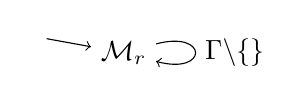
\begin{tikzpicture}
   \node (0) at (0,0) {$\M_r$};
   \node (init) at (-1.1,.2) {};
   \draw[->] (init) to (0);
   \draw[->,loop right] (0) to node {$\Gamma\backslash\{\blank\}$} (0);
  \end{tikzpicture}

  
  \item Linksmaschine $\M_L$:
  
  Geht für beliebigen Bandinhalt nach links, bis ein Blanksymbol erreicht ist, und hält dann.
  Es wird mindestens ein Schritt gemacht.

  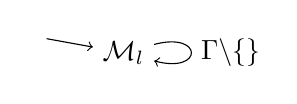
\begin{tikzpicture}
   \node (0) at (0,0) {$\M_l$};
   \node (init) at (-1.1,.2) {};
   \draw[->] (init) to (0);
   \draw[->,loop right] (0) to node {$\Gamma\backslash\{\blank\}$} (0);
  \end{tikzpicture}
  \qedhere
 \end{itemize}
\end{Bsp}

Wir definieren das Flussdiagramm nun formal wie folgt.


\begin{Def}[name={[Flussdiagram]}]
Ein \emph{Flussdiagramm} ist ein 8-Tupel $G=(\Sigma, \Gamma, \blank,V,E,v^\mathsf{init},L_V,L_E)$.
Dabei ist
\begin{itemize}
 \item $\Sigma$ ein Alphabet, das wir \emph{Eingabealphabet} nennen,
 \item $\Gamma\supsetneq \Sigma$ ein Alphabet, das wir \emph{gemeinsames Bandalphabet} nennen,
 \item $\blank\in \Gamma\setminus\Sigma$ ein Zeichen, das wir \emph{gemeinsames Blanksymbol} nennen,
 \item $(V,E)$ ein gerichteter Graph,
 \item $v^\mathsf{init}\in V$ ein Knoten, den wir \emph{Startknoten} nennen,
 \item $L_V$ eine Abbildung, die jedem Knoten $v \in V$ eine Turingmaschine zuordnet und
 \item $L_E: E \to \Powerset(\Gamma)$ eine Abbildung, die jeder Kante $(v,v')\in E$ eine Teilmenge des Bandalphabets zuordnet.
 \qedhere
\end{itemize}
\end{Def}


Notation: Bis zum Ende des Kapitels schreiben wir
$\M_v=\left(\Sigma,Q_v,\Gamma,\delta_v,\qinit_v,\blank,F_v\right)$
für die Turingmaschine $L_V(v)$, also die Turingmaschine, die dem Knoten $v$ zugeordnet ist.

\begin{Def}[name={[Von Flussdiagram definierte \ac{TM}]}]
Die von einem Flussdiagramm $G=(\Sigma, \Gamma, \blank,V,E,v^\mathsf{init},L_V,L_E)$ definierte Turingmaschine ist 
$\M=\left(\Sigma,Q,\Gamma,\delta,\qinit,\blank,F\right)$, wobei
\begin{itemize}
 \item $Q=\overset{.}{\bigcup\limits_{v\in V}} Q_v$~~\footnote{Um eine disjunkte Vereinigung zu erreichen, müssen wir ggf.\ Zustände umbenennen.}
 \item $\qinit = \qinit_{v^\mathsf{init}}$
 \item $\delta(q,x) = 
 \begin{cases}
 \delta_v(q,x) & \text{falls } q\in Q_v \text{ und }  \delta_v(q,x)\neq\emptyset \\[4mm]
 \left\{(q'',x,N) \,\middle|\, \begin{array}{@{}l@{\,}}
       q\in Q_v, (v,v')\in E,\\
       x\in L_E((v,v')), q''=\qinit_{{v'}}
      \end{array}\right\} & \text{sonst }
 \end{cases}$
 \item $F=\overset{.}{\bigcup\limits_{v\in V}} F_v$.
 \qedhere
\end{itemize}
\end{Def}

Konvention: Analog zu Startzuständen von endlichen Automaten verwenden wir einen eingehenden Pfeil, um den Startknoten eines Flussdiagramms zu kennzeichnen.

\begin{Bsp}\datenote{11.01.2019}
Wir wollen eine \ac{TM} konstruieren, welche die wie folgt definierte Subtraktion von natürlichen Zahlen implementiert.
% 
% mit Hilfe eines Flussdiagramms eine .
% 
$$
f: \N\times\N\rightarrow \N
\qquad \qquad
f(x,y)=
\begin{cases}
 x - y & \text{ falls } x\geq y\\
 0  & \text{ sonst}
\end{cases}
$$

Wir verwenden dabei eine auf Strichsymbolen basierende Unärcodierung für die Operanden
und nehmen an, dass das Zeichen $\#$ verwendet wird, um die Operanden $x$ und $y$ in der Eingabe zu trennen.
Wir haben also $\Sigma=\{I,\#\}$ und für Minuend $x$ und Subtrahend $y$ hat die Eingabe hat die folgende Form. 
$$\underbrace{I\ldots I}_{x\text{ Mal}}\#\underbrace{I\ldots I}_{y\text{ Mal}}$$


Idee: Lösche für jeden $y$-Strich einen $x$-Strich.
Lösche falls nötig (Fall $y>x$) verbleibende $y$-Striche. Lösche anschließend das Trennzeichen~$\#$.
Wir verwenden die übliche Notation für das Blanksymbol, 
benötigen keine weiteren Zeichen für unsere Berechnung und verwenden daher das Bandalphabet $\Gamma:=\Sigma\cup\{\mblank\}$.

  \begin{center}
  \begin{tikzpicture}
   \node (0) at (0,0) {$\M_R$};
   \node (init) at (-1.1,.2) {};
   \node[right= of 0] (1) {$\M_l$};
   \node[right= of 1] (2) {$\D_\mblank$};
   \node[right= of 2] (3) {$\M_L$};
   \node[right= of 3] (4) {$\M_r$};
   \node[right= of 4] (5) {$\D_\mblank$};
   
   \node[below= of 4] (6) {$\D_\mblank$};
   \node[right= of 6] (7) {$\M_r$};
   \node[below= of 1] (9) {$\D_\mblank$};
%    \node[right= of 9] (10) {$\M_L$};
   
   \draw[->] (init) to (0);
   \draw[->] (0) to node[auto] {$\Gamma$} (1);
   \draw[->] (1) to node[auto] {$\{I\}$} (2);
   \draw[->] (2) to node[auto] {$\Gamma$} (3);
   \draw[->] (3) to node[auto] {$\Gamma$} (4);
   \draw[->] (4) to node[auto] {$\{I\}$} (5);
   \draw[->, in=90, out=90, looseness=0.4] (5) to node[auto] {$\Gamma$} (0);
   \draw[->] (4) to node[auto] {$\{\#\}$} (6);
   \draw[->] (6) to node[auto] {$\Gamma$} (7);
   \draw[->, in=-90, out=-90, looseness=0.6] (7) to node[auto] {$\{I\}$} (6);
   \draw[->] (1) to node[auto] {$\{\#\}$} (9);
%    \draw[->] (9) to node[auto] {$\Gamma$} (10);
  \end{tikzpicture}
  \end{center}
  
  Die obere Schleife beschreibt das simultane Entfernen von Strichen in $x$ und $y$.
  Die erste Abzweigung nach unten wird genommen, wenn alle Striche von $y$ entfernt wurden -- also ursprünglich $y$ kleiner ($\leq$) als $x$ war.
  Die untere Schleife wird ausgeführt, wenn $y$ echt größer als $x$ war; sie dient dazu, die verbleibenden Zeichen auf dem Band zu löschen,
  um die unärcodierte $0$ (also das leere Wort) zu erzeugen.
\end{Bsp}
  
\subsection{Varianten von \ac{TM}s}
Es gibt viele Varianten von Turingmaschinen.
Diese sind typischerweise äquivalent zu \autoref{def:4.tm} in dem Sinne, dass sie die gleiche Klasse von Sprachen akzeptieren und die gleiche Menge von Funktionen berechnen können.
Welche Variante am bequemsten zu benutzen ist, hängt von der Anwendung ab.
Wir stellen in diesem Unterkapitel zwei alternative Varianten von TMs vor.
Die Beschreibungen der Maschinen, die Behauptungen und zugehörigen Beweisskizzen sind in diesem Unterkapitel eher informell gehalten.
Wir ermutigen die Leserschaft darüber nachzudenken wie man die Inhalte analog zu den vorigen Kapiteln formal präsentieren könnte.


\subsubsection{Mehrspurmaschinen}

Eine $k$-Spur-Turingmaschine arbeitet wie eine (gewöhnliche) \ac{TM}, aber das Band hat hier $k$ Spuren.
Der Kopf liest und schreibt also immer einen $k$-Vektor von Zeichen.
Die Transitionsfunktion hat den Typ $\delta: Q\times\Gamma^k\--> \Powerset(Q\times\Gamma^k\times\{R,L,N\})$.

Die Eingabe steht zu Beginn auf der ersten Spur.
Zum Ermitteln der Ausgabe betrachten wir auch nur die erste Spur.

	\begin{figure}[H]\centering
		{\renewcommand{\arraystretch}{0.8}
		\begin{tabu} to .5\textwidth {X[.35]|X[.65]}
			&\\\hline
			&\\\hline
			&\\\hline
			&\\\hline
			&
		\end{tabu}}
		\caption{Mehrspurmaschine}
	\end{figure}

	\begin{Bsp*}
		binäre Addition und Multiplikation nach der Schulmethode
	\end{Bsp*}

\begin{Bemerkung}
Eine $k$-Spur-\ac{TM} kann von einer (gewöhnlichen) \ac{TM} simuliert werden.

\medskip

Idee: Verwende Bandalphabet $\Gamma_\mathsf{sim} = \Sigma \overset{.}{\cup} (\Gamma^k\times\{\blank, B\})\text{ und Blanksymbol } \blank_\mathsf{sim}=\blank^{k+1}$.
Hierbei steht $B$ für "`besucht"'.

\begin{enumerate}
 \item Konvertieren der Eingabe:
 
 Laufe einmal über die Eingabe und ersetze $a\in\Sigma$ durch $\left(\begin{array}{c}a\\ \mblank\\ \vdots\\ \mblank\end{array}\right)\in\Gamma_\mathsf{sim}$.
 Bewege den Kopf zurück in die Ausgangsposition (also die am weitesten links liegende Zelle, die verschieden von $\blank_\mathsf{sim}$ ist).
 
 \item Simulation:
 
 Exaktes Nachahmen jedes Rechenschritts der $k$-Spur-\ac{TM}, bis diese anhält.
 Schreibe dabei als $k+1$-te Komponente des Tupels immer ein $B$.
 
 \item Konvertieren der Ausgabe:
 
 Idee: Ersetze jedes $\left(\begin{array}{c}a_1\\ \vdots\\ a_k\\ x\end{array}\right)\in\Gamma_\mathsf{sim}$ durch $a_1$, falls $a_1\in\Sigma$, und sonst durch
 $\left(\begin{array}{c}\mblank \\ \mblank\\ \vdots\\ \mblank\end{array}\right)$.
 (Zur Ausgabe gehören schließlich nur die Elemente aus $\Sigma$.)
 
	Problem: Woher wissen wir, wie weit wir nach rechts laufen müssen?
  
  Lösung: Wir achten auf die letzte Komponente des Tupels. 
  Wir laufen so lange nach rechts, wie dort ein B steht, denn alle diese Zellen haben wir mindestens einmal besucht.
  
 \qedhere
\end{enumerate}
\end{Bemerkung}



\subsubsection{Mehrbandmaschinen}

Eine $k$-Band-\ac{TM} hat $k$ Bänder, die jeweils einen eigenen Kopf haben.
In jedem Schritt wird jeder Kopf lesen, schreiben und sich bewegen.
Dabei darf sich jeder Kopf in eine andere Richtung bewegen.

Die Transitionsfunktion hat den Typ $\delta: Q\times\Gamma^k\--> \Powerset(Q\times\Gamma^k\times\{R,L,N\}^k)$.


\begin{Bemerkung}
Eine $k$-Band-\ac{TM} $\M$ kann von einer $2k+1$-Spur-\ac{TM} $\M_\mathsf{sim}$ simuliert werden.

\medskip

Idee: Codiere die Konfiguration einer $k$-Band-\ac{TM} mit Hilfe von $2k$ Spuren.
Simuliere einen Schritt der $k$-Band-\ac{TM} in mehreren Schritten.
Verwende dabei eine zusätzliche Spur, um das bisher bearbeitete Band zu kennzeichnen.
Der Zustand von $\M$ wird im Zustand von $\M_\mathsf{sim}$ codiert.

Das Bandalphabet der $k$-Spur-\ac{TM} sei dabei $\Gamma_\mathsf{sim}=\Gamma\overset{.}{\cup}\{\#,B\}$.

		\begin{itemize}
			\item Spur $2i-1$ simuliert Band $i$.
			\item Spur $2i$ ist leer bis auf einen Marker \#, welcher die Position des Kopfs auf Band $i$ markiert.
			\item Spur $2k+1$ enthält das Zeichen $B$ an jeder Position, die bereits bearbeitet wurde.
		\end{itemize}
		
	\begin{tabular}{lll}
		Spur\\
		1 & \ruleplaceholder[ Band 1 ]{.5\linewidth}\\
		2 & \hspace{.23\linewidth}\# Kopf für Band 1\\
		3 & \ruleplaceholder[ Band 2 ]{.5\linewidth}\\
		4 & \multicolumn1r{\# Kopf 2\qquad\ }\\
		& \hspace*{35mm} \vdots\\
		$2k-1$ & \ruleplaceholder[ Band k ]{.5\linewidth}\\
		$2k$ & \hspace*{1cm} \# Kopf $k$\\
		$2k+1$ & \ldots\ \blank\  \blank\  B\ B\ B\ B\ \ \ \ \ldots \ \ \ B\ B\ B\ B\ \blank\  \blank \ \ldots  \\
		& \hspace{11mm} $\uparrow$ linker Rand \hspace{18mm} $\uparrow$ rechter Rand
	\end{tabular}
	\begin{enumerate}
	 \item Herstellen der Start-Konfiguration:
	 
	 \begin{itemize}
	  \item Schreibe Kopfmarkierung (Zeichen \#) auf allen geraden Spuren und $B$ auf Spur $2k+1$.
	  
	  	\begin{tabular}{*2{M{l}}}
		\text{Spur }1 & a_1a_2\dots a_n~~(= \text{Eingabe})\\
		2 & \#\\
		3 & \blank\\
		4 & \#\\
		\vdots\\
		2k-1 & \blank\\
		2k & \#\\
		2k+1 & \blank B \blank
	\end{tabular} 
	 \end{itemize}
	 
    \item Simulation:

	Der Kopf der Mehrspurmaschine startet jeweils bei der linken Begrenzung, also beim am weitesten links stehenden $B$ auf Spur $2k+1$.
	\begin{itemize}
		\item Laufe bis zum rechten Rand.
		Sammle dabei die Symbole unter den Köpfen (markiert mit \#) und merke dir diese im Zustand (Vektorcodierung $\overrightarrow{\gamma} \in \Gamma^k$).
		\item Bestimme Resultat von Transitionsfunktion $\delta(q,\overrightarrow{\gamma})=(q',\overrightarrow{\gamma'},\overrightarrow{d})$\\
		neuer Zustand $q'$, für jeden Kopf ein neues Symbol $\overrightarrow{\gamma'}$ und Richtung $\overrightarrow{d}$.
		\item Laufe zurück nach links.
		Schreibe dabei das jeweilige Zeichen $\overrightarrow{\gamma}'$ am entsprechenden Kopf und versetze diesen gemäß $\overrightarrow{d}$.
	\end{itemize}
	Falls eine Kopfbewegung den Rand auf Spur $2k+1$ überschreitet, dann schreibe ein weiteres $B$.
	
	Beim Rücklauf: Teste auf Haltekonfiguration der $k$-Band-\ac{TM}.
	Falls ja, so springe in eine Haltekonfiguration der $k$-Spur-\ac{TM}.
% 	
% 	Weiter im Zustand Sim$(q')$.
	\qedhere
	\end{enumerate}
\end{Bemerkung}


\begin{Bemerkung}
	Angenommen, für ein Wort der Länge $n$ benötige die $k$-Band-\ac{TM} $\M\ T(n)$ Schritte und $S(n)$ Zellen auf den Bändern.
	Dann benötigt $\M_\mathsf{sim}$ höchstens $O(S(n))$ Zellen und $O(S(n)\cdot T(n))=O(T(n)^2)$ Schritte.
\end{Bemerkung}





\subsection{Universelle Turingmaschine}\datenote{16.01.2019}
Die bisher betrachteten Turingmaschinen waren (ebenso wie endliche Automaten oder Kellerautomaten) 
auf einen Einsatzzweck beschränkt und konnten nur eine bestimmte Sprache akzeptieren oder eine bestimmte Funktion berechnen.
Dies entspricht nicht unserer Vorstellung eines Computers, denn dieser kann normalerweise beliebige Programme ausführen.

In diesem Kapitel konstruieren wir nun eine \ac{TM} $\M_U$, die als Eingabe sowohl
eine Codierung $\godel{\M}$ einer beliebigen \ac{TM} $\M$ als auch deren Eingabe $w$ nimmt, sodass die folgenden drei Eigenschaften gelten.
\begin{align}
	\label{Mu-eq-lang} w\in L(\M) &\Leftrightarrow \godel{\M}\#w \in L(\M_U)\\
	\label{Mu-eq-term} \text{$\M$ hält auf Eingabe $w$} &\Leftrightarrow \text{$\M_U$ hält auf Eingabe $\godel{\M}\#w$}\\
	\label{Mu-eq-func} \text{$f_\M(w)$} &= \text{$f_{\M_U}(\godel{\M}\#w)$}
\end{align}

Wir nennen $\M_U$ die \emph{universelle Turingmaschine}.

\subsubsection{Codierung von Turingmaschinen}\label{subsec:codeTuring}

Zunächst wollen wir uns eine Codierung $\godel{\M}$ für $\M=(\Sigma, Q, \Gamma, \delta, \qinit, \blank, F)$ überlegen.
Die Effizienz unserer Codierung ist uns dabei nicht wichtig und wir versuchen der Einfachheit wegen mit Unärcodierungen zu arbeiten.

Uns ist nicht wichtig dass alle Details von $\M$ codieren uns ist nur wichtig, 
dass wir eine \ac{TM} mit dem Verhalten von $\M$ codieren. 
Deshalb können wir uns mit den folgenden Überlegungen die Codierung vereinfachen.
\begin{itemize}
	\item Da $Q$ und $\Gamma$ endlich sind, können wir jedem ihrer Elemente eine natürliche Zahl zuordnen
	und in der Codierung dann nur diese Zahl verwenden.
	\item Wir müssen $\qinit$ und $\blank$ nicht explizit codieren; wir verwenden die Konvention,
	dass $\qinit$ der Zustand mit der Nummer $1$ und $\blank$ das Zeichen mit der Nummer $1$ ist.
	\item Wir müssen $\Sigma$, $Q$ und $\Gamma$ nicht explizit in die Codierung mit aufnehmen.
	Für das Ausführen einer \ac{TM} sind nur die Elemente aus $\Sigma$, $Q$ und $\Gamma$ relevant, die auch in der Transitionsfunktion $\delta$ vorkommen.
\end{itemize}

\newcommand{\tmach}{\ensuremath{\mathbb{M}}}

{\color{green!50!black}
Wir möchten einer Konvention und der darauf folgenden Definition dafür sorgen dass wir die obigen Überlegungen umsetzen können.
\footnote{In der Vorlesung vom 16.01.2019 gab es Fragen zur Umsetzung einer eindeutigen Codierung von \acp{TM}.
	Ich habe deshalb diesen grünen Text nachträglich hinzugefügt und die Definition der \emph{normierten \ac{TM}} in der Vorlesung vom 18.01.2019 vorgestellt. }

\textbf{Konvention: } 
Wir wollen von nun an ein Alphabet $\Sigma=\{a_1,\ldots, a_{n_\Sigma}\}$ festhalten.
Somit ist immer wenn wir von der Folge $a_1,\ldots, a_{n_\Sigma}$ sprechen die gleiche Reihenfolge der Symbole gemeint.


Seien $q_1,q_2,\ldots$ und $b_1,b_2,\ldots$ zwei unendlich lange Folgen die jeweils für jede positive natürliche Zahl ein Element enthalten.
In der folgenden Definition werden wir endliche Präfixe dieser Folgen als Zustände bzw. Symbole des Bandalphabets verwenden.

\begin{Def}[name={[normierte \ac{TM}]}]\label{def:normTM}
	Wir nennen eine \ac{TM} $\M=(\Sigma, Q, \Gamma, \delta, \qinit, \blank, F)$  \emph{normiert} falls
	\begin{itemize}
		\item $Q=\{q_1,\ldots, q_{|Q|}\}$
		\item $\Gamma=\{b_1,\ldots b_{|\Gamma|-|\Sigma|}, a_1,\ldots a_{n_\Sigma}\}$
		\item $\qinit = q_1$
		\item $\blank = b_1$
		\item Für alle $q\in Q$ existiert ein $x\in\Gamma$ sodass $\delta(q,x)\neq\{\}$\footnote{
			Anschaulich: Jeder Zustand kommt mindestens ein mal in der Turingtablle vor.}
		\item Für alle $x\in\Gamma\setminus(\Sigma\cup\{\mblank\})$ existiert ein $q\in Q$ sodass $\delta(q,x)\neq\{\}$.\footnote{
			Anschaulich: Jedes Symbol des Bandalphabetes ist entweder das Blank, Teil der Eingabealphabetes oder es kommt mindestens ein mal in der Turingtablle vor.}
	\end{itemize}
	Wir schreiben $\mathbb{M}$ für die Menge aller normierten \ac{TM}s.
\end{Def}



\begin{lemma}
	Für Zu jeder TM $\M$ existiert eine normierte TM $\M'$ dass
	\begin{itemize}
		\item $f_{\M'}=f_{\M}$
		\item $L(\M')=L(\M)$
	\end{itemize}
\end{lemma}
\begin{proof}
	Umbenennen und Löschen von Zuständen und Symbolen des Bandalphabetes.
\end{proof}
}



Idee: Codiere Elemente aus $Q$ und $\Gamma$ unär mit dem Zeichen~$0$.
Verwende das Zeichen~$1$, um unärcodierte Zahlen zu trennen.

\begin{itemize}
 \item Zustände:
 
    Seien $q_1,\dots, q_{n}$ die Elemente von $Q$, sodass $q_1=\qinit$.
    
    Definiere $\godel{q_i}:=0^i$.
    
  \item Menge der akzeptierenden Zustände:
  
    Seien $q_{k_1},\dots, q_{k_n}$ die Elemente von $F$, in der Reihenfolge sodass $k_1<\ldots <k_n$ gilt.
    
    Definiere $\godel{F}:=\godel{q_{k_1}} 1 \godel{q_{k_2}} 1 \ldots 1 \godel{q_{k_n}}$.
    
  \item Bandalphabet:
  
    Seien $b_1,\dots, b_{n}$ die Elemente von $\Gamma$, sodass $b_1=\blank$.
    
    Definiere $\godel{b_j}:=0^j$.
    
  \item Richtung (in die der Schreib-Lesekopf bewegt wird):
  
    Definiere $\godel{L}:=0$, $\godel{N}:=00$ und $\godel{R}:=000$.
    
  \item Transitionsfunktion:
  
   Seien $(q_{t_1}, b_{t_1}, q_{t_1}', b_{t_1}', d_{t_1}),\dots, (q_{t_n}, b_{t_n}, q_{t_n}', b_{t_n}', d_{t_n})$ 
   die Elemente von $\delta$, die nicht auf $\{\}$ abgebildet werden.
   Diese Elemente seien durch eine lexikographische Sortierung gegeben
  
   Definiere
   
   $\godel{\delta}:= \godel{q_{t_1}}1\godel{a_{t_1}}1\godel{q_{t_1}'}1\godel{a_{t_1}'}1\godel{d_{t_1}}11\dots 11 \godel{q_{t_n}}1\godel{a_{t_n}}1\godel{q_{t_n}'}1 \godel{a_{t_n}'}1\godel{d_{t_n}}$.
   
   \item Turingmaschine:
   
   $\godel{\M}:=111\godel{\delta}111\godel{F}111$
\end{itemize}


\begin{Bsp}\label{bsp:CodeVonMr}
	Wir bestimmen nun die Codierung $\godel{\M_r}$ der 1-Schritt-Rechtsmaschine aus \autoref{bsp:simpletms} für $\Sigma = \{0, 1\}$ und $\Gamma = \{0, 1, \blank\}$.
	Wir nehmen dabei für die Elemente von $Q$, $\Gamma$ und $\delta$ die folgenden Reihenfolgen an.
	
	\begin{center}
	\begin{tabular}{c|l}
    $Q$ & $q_0,q_1$\\ \hline
    $\Gamma$ & $\blank, 0, 1$\\ \hline
    $\delta$ & $(q_0, \blank, q_1, \blank, R), (q_0, 0, q_1, 0, R), (q_0, 1, q_1, 1, R)$
	\end{tabular}
	\end{center}
	Wir erhalten:
	\begin{itemize}
		\item Zustände: $\godel{q_0} = 0, \godel{q_1} = 00$
		
		\item Menge der akzeptierenden Zustände: $\godel{F} = \Eps$ (da $F = \{\}$)
		
		\item Bandalphabet: $\godel{\blank} = 0$, $\godel{0} = 00$, $\godel{1} = 000$
	
		\item Turingmaschine: $\godel{\M_r}$ = \\ $111 \underbrace{\overbrace{0\,1\,0\,1\,00\,1\,0\,1\,000}^\text{erste Transition} 11 \overbrace{0\,1\,00\,1\,00\,1\,00\,1\,000}^\text{zweite Transition} 11 \overbrace{0\,1\,000\,1\,00\,1\,000\,1\,000}^\text{dritte Transition}}_{\godel{\delta}}111\underbrace{\,}_{\godel{F}}111$
		\qedhere
	\end{itemize}
\end{Bsp}



\subsubsection{Arbeitsweise der universellen Turingmaschine}
Da die universelle Turingmaschine $\M_U$ recht komplex ist, wollen wir diese hier nicht formal definieren, sondern geben nur eine informelle Beschreibung der Arbeitsweise an.


Wie definiere $\M_U$ als 3-Band-\ac{TM}, wobei die Bänder $B_1$, $B_2$ und $B_3$ wie folgt genutzt werden.
\begin{itemize}
\item[$B_1:$] Zu Beginn steht hier die Eingabe für $\M_U$.
Nach der Initialisierung von $\M_U$ verwenden wir $B_1$, um das Band der Eingabeturingmaschine $\M$ nachzuahmen.
\item[$B_2:$] Speichere die Codierung der Eingabeturingmaschine $\ulcorner \M \urcorner$.
\item[$B_3:$] Speichere den aktuellen Zustand von $\M$ ($0^k$ für Zustand $q_k$).
\end{itemize}

Die universelle Turingmaschine $\M_U$ beginnt zunächst mit einer Initialisierung, die aus den folgenden drei Teilen besteht.

\begin{enumerate}
 \item Prüfe, ob der erste Teil der Eingabe $\ulcorner \M \urcorner$ eine gültige Turingmaschine codiert.
 
 Die Menge der gültigen Codierungen kann mit Hilfe einer kontextfreien Grammatik beschrieben werden (siehe Übungen).
 
 \item Verschiebe $\ulcorner \M \urcorner$ auf $B_2$. Schreibe dabei Blanksymbole auf die Bandzellen von $B_1$.
 Überschreibe anschließend das Symbol $\#$, das die Eingabeturingmaschine und das Eingabewort trennt, durch ein Blanksymbol.
 
 \item Schreibe $0$ (also die Codierung des Startzustands von $\M$) auf $B_3$.
\end{enumerate}

Nach der Initialisierung ist $\M_U$ also in der folgenden Konfiguration.
\begin{itemize}
\item[$B_1:$] $w$
\item[$B_2:$] $\ulcorner \M \urcorner$
\item[$B_3:$] $0$
\end{itemize}

Nach der Initialisierung wird $\M_U$ das Verhalten von $\M$ nachahmen.
Für jeden Schritt von $\M$ macht $\M_U$ dabei die folgenden Schritte.

 Suche ein Element $(q, a, q', a', d)$ der Transitionsfunktion $\delta$ von $\M$, das zum aktuellen Zustand $q$ und zum aktuellen Bandsymbol $a$ passt.
 
 Wir laufen hierfür einmal über das komplette Band $B_2$. 
 Zustände werden zeichenweise mit dem Inhalt von $B_3$ verglichen.
 Die Zuordnung von Alphabetsymbolen $a$ zur Codierung $\godel{a}$ ist fest in $\M_U$ eingebaut.
 
 \begin{itemize}
 
 \item Falls solch ein Element der Transitionsfunktion existiert,
    schreibe auf $B_1$ das Zeichen $a'$ und bewege den Kopf wie durch $d$ definiert.
    Ersetze außerdem die Codierung $\godel{q}$ auf $B_3$ durch $\godel{q'}$.
    Fahre anschließend mit dem Nachahmen des nächsten Schritts von $\M$ fort.
    
 \item Falls kein solches Element der Transitionsfunktion existiert, hat $\M$ eine Haltekonfiguration erreicht.
 Wir vergleichen nun den aktuellen Zustand (auf $B_3$) mit den auf $B_2$ gespeicherten akzeptierenden Zuständen und akzeptieren oder verwerfen die Eingabe entsprechend.

\end{itemize}

\begin{Satz}[name={[Universelle \ac{TM}]}]
	Die universelle \ac{TM} $\M_U$ erfüllt die Eigenschaften (\ref{Mu-eq-lang}), (\ref{Mu-eq-term}) und (\ref{Mu-eq-func}).
\end{Satz}


%%% Local Variables:
%%% mode: latex
%%% TeX-master: "Info_3_Skript_WS2016-17"
%%% End:
